\chapter{Números irracionales}

¿Por qué es tan importante el teorema de Pitágoras?  El teorema 
introduce naturalmente números irracionales. La hipotenusa de un triángulo
rectángulo cuyos lados miden uno es igual a $\sqrt{2}$, un número cuyo cuadrado
es dos.  En tiempos de Pitágoras esto se mantuvo en secreto ya que no era un
resultado que pudiera comprenderse totalmente. Los pitagóricos
no podían aceptar que $\sqrt{2}$ fuera un número, aunque supieran que $\sqrt{2}$ es
la diagonal de un cuadrado unitario. Las cantidades geométricas
eran entonces, en general, tratadas de forma que no fuera necesario utilizar números. La
relación entre aritmética y geometría estaba parcialmente rota. Sin embargo,
para solventar las dificultades originadas por esta división, los griegos
desarrollaron entonces ingeniosos métodos para entender cuánto podría
aproximarse una cierta cantidad geométrica en términos de números racionales.
Podemos encontrar estas ideas en el libro X de los Elementos, donde Euclides
estudia detalladamente números de la forma
\[
	\sqrt{\sqrt{a}\pm\sqrt{b}}
\]
donde $a$ y $b$ son números racionales. 

Durante muchos años la matemática no vio avances en relación con los números
irracionales, salvo, quizá, la observación que hizo Fibonacci en 1225 sobre la
irracionalidad de las soluciones de la ecuación 
\[
	x^3+2x^2+10x=20.
\]
Fibonacci demostró que las soluciones son números irracionales, pero no esos
irracionales estudiados por Euclides en el libro X. 

Las ideas sobre irracionales de la matemática griega fueron redescubiertas por
Dedekind en el siglo XIX y permitieron que la aritmética y la geometría
finalmente pudieran convivir pacíficamente.

\begin{exercise}
	Demuestre que un entero $m$ es par si y sólo si $m^2$ es par.
\end{exercise}

La demostración de la irracionalidad de $\sqrt{2}$ que daremos a continuación
aparece en uno de los libros de Aristóteles.

\begin{theorem}
	El número $\sqrt{2}$ no es racional.	
\end{theorem}

\begin{proof}
	Si suponemos que $\sqrt{2}=a/b$ con $a$ y $b$ son números naturales sin
	factores en común, entonces $(a/b)^2=2$. Esto implica que $a^2=2b^2$ es un
	número par. Luego $a$ es par, digamos $a=2c$. Entonces $2b^2=a^2=4c^2$
	implica que $b^2=2c^2$ y luego $b$ es par, una contradicción.
\end{proof}

% agregar los ejercicios del libro de rey pastor y Babibi
% ver si hay algo interesante en stillwell
La demostración que vimos usa fuertemente la paridad de los números naturales.
Gracias a uno de los diálogos de Platón sabemos que el matemático griego
Teodoro estudió algunos números irracionales y demostró la irracionalidad de
$\sqrt{n}$ para los $n<17$ que no son cuadrados. Se nos dice además que Teodoro
concibió la figura~\ref{fig:teodoro} y que justamente fue en el número 17 donde
su análisis se detuvo. 

\begin{figure}[h]
		\centering
		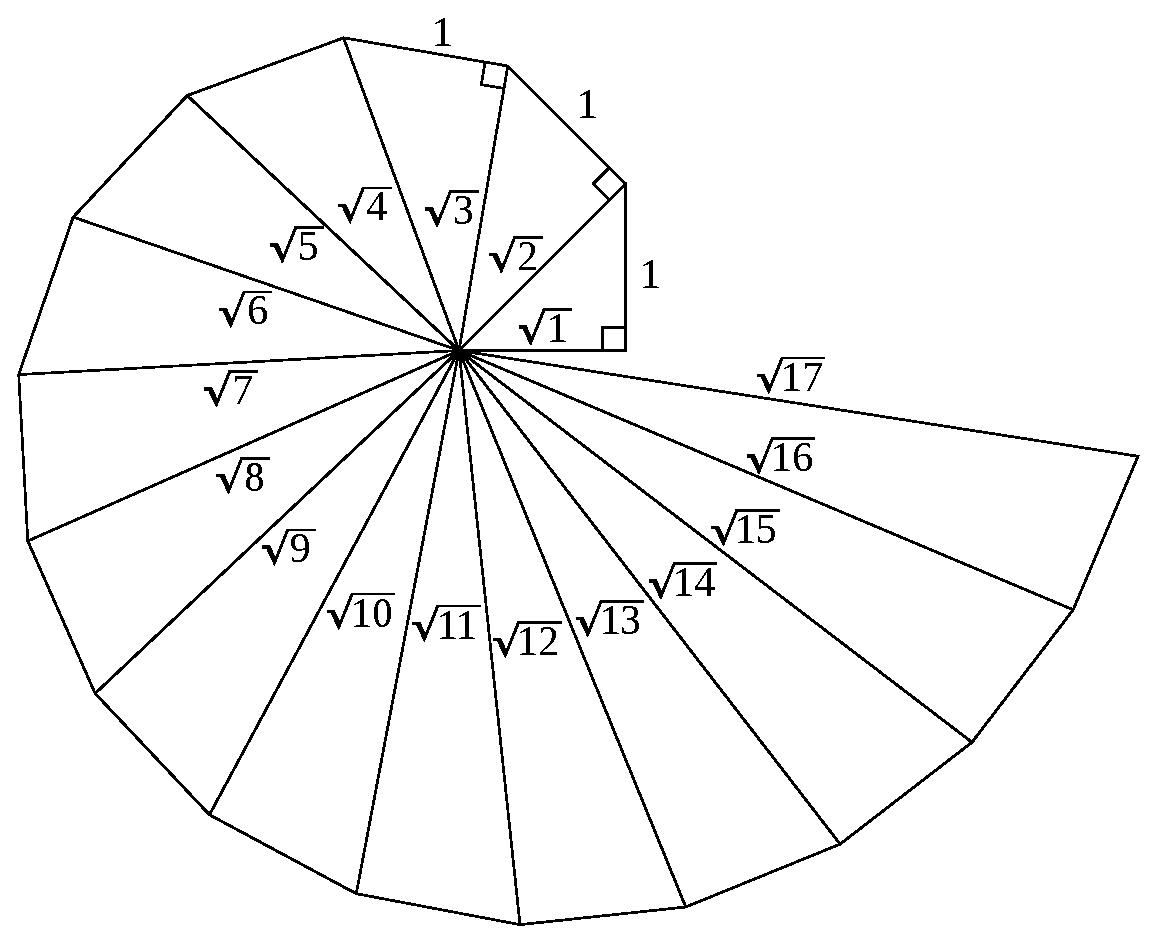
\includegraphics[scale=0.3]{images/teodoro}
		\caption{La espiral de Teodoro.}
		\label{fig:teodoro}
\end{figure}

No se sabe exactamente qué demostraciones encontró
Teodoro. Más interesante fue para los historiadores saber por qué Teodoro se
detuvo justamente en $17$. Algunos creen que fue porque a partir de ese número
el dibujo que vemos en la figura~\ref{fig:teodoro} tiene superposiciones, aunque
esta versión no parece ser una explicación suficientemente fuerte 
como para convencernos. De hecho, en 1958 se demostró que esas supuestas superposiciones 
son fácilmente evitables si extendemos la espiral tal como vemos en la
figura~\ref{fig:espiral_infinita}.  

\begin{figure}[h]
		\centering
		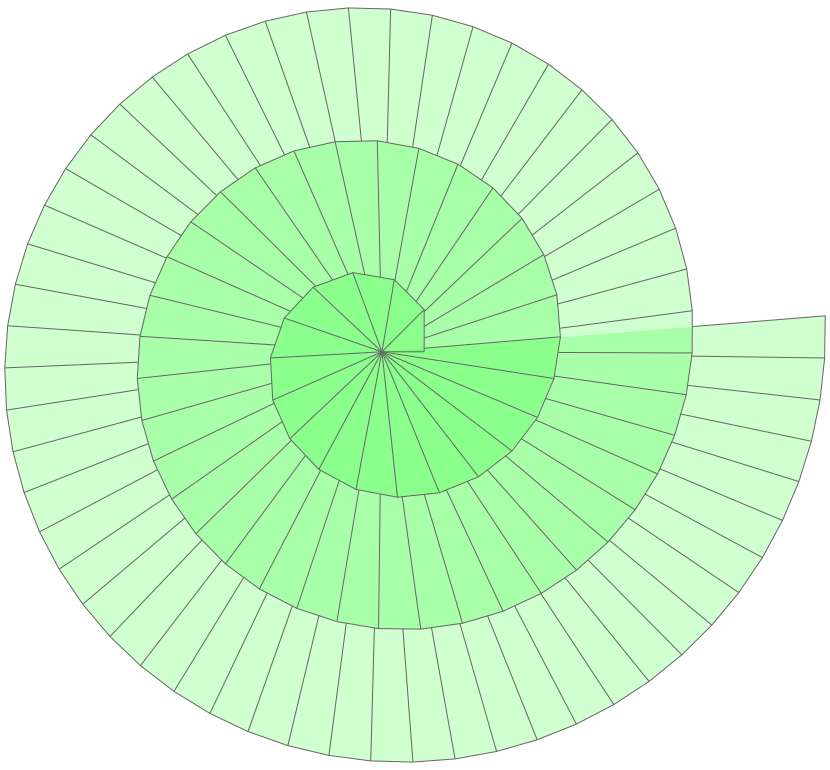
\includegraphics[scale=0.2]{images/infinita}
		\caption{Una extensión de la espiral de Teodoro.}
		\label{fig:espiral_infinita}
\end{figure}

Una explicación más razonable --observada
por Heath en 1931-- se basa en el siguiente hecho: la técnica basada en el uso
de la paridad falla por primera vez justamente en 17.  Supongamos que
$\sqrt{17}=a/b$, donde $a$ y $b$ son coprimos; entonces $17b^2=a^2$. Como $a$ y
$b$ son coprimos, ambos son impares, digamos $a=2k+1$ y $b=2l+1$. Al reemplazar
obtenemos entonces
\[
	17(4l^2+4l+1)=4k^2+4k+1,
\]
que al simplificarse queda $17l(l+1)+4=k(k+1)$. ¡Aquí no hay contradicción!

Tal como se afirma en~\cite{MR0416824}, muy probablemente esta sea la razón por
la que Teodoro detuvo su análisis en 17. No nos olvidemos que los griegos
creían fuertemente en la potencia de las técnicas de paridad. De hecho, para
Platón la aritmética era la teoría de los pares y los impares. 

Veamos ahora que el argumento de paridad sí funciona para números menores que
17 que no son cuadrados. Este resultado será consecuencia de un resultado mucho
más general:

\begin{theorem}
	Si $n$ es un entero positivo que puede escribirse como $4m+2$, $4m+3$,
	$8m+5$, entonces puede demostrarse que $\sqrt{n}$ es irracional con un
	argumento de paridad.
\end{theorem}

\begin{proof}
	Consideremos el caso $n=8m+5$ y escribamos $\sqrt{8m+5}=a/b$, donde $a$ y
	$b$ son coprimos. Como $(8m+5)b^2=a^2$, tanto $a$ como $b$ deberán ser
	números impares. Escribimos entonces $a=2k+1$ y $b=2l+1$ y reemplazamos
	para obtener 
	\[
		(8m+5)(l^2+l)+(2m+1)=k^2+k,
	\]
	una contradicción pues $2m+1$ es impar y los números $k^2+k$ y
	$l^2+l$ son ambos números pares.  Los dos casos restantes son
	similares. 
\end{proof}

Como sabemos que $\sqrt{2}$ es irracional, también será irracional
$\sqrt{8}=2\sqrt{2}$.  Similarmente, si demostramos la irracionalidad de
$\sqrt{3}$ tendremos también demostrada la irracionalidad de $\sqrt{12}$ pues
$\sqrt{12}=2\sqrt{3}$. Como
\begin{align*}
	&3=4\times 0+3, 
	&&4=2^2,
	&& 5=8\times 0+5,
	&& 6=4\times 1+2,\\
	& 7=4\times 1+3,
	&& 9=3^2,
	&& 10=4\times 2+2,
	&& 11=4\times 2+3,\\
	& 13=8\times 1+5,
	&& 14=4\times 3+2,
	&& 15=4\times 3+3.
	&& 16=4^2,
\end{align*}
vemos que todos los números menores a 17 que no son cuadrados perfectos quedan
cubiertos por el teorema. 

%En las últimas versiones, por ejemplo~\cite{MR2445243}, Hardy y Wright\dots


%\begin{exercise}
%	Demuestre que $\sqrt{17}$ es un número irracional.
%\end{exercise}

Terminaremos nuestra discusión sobre números irracionales con el siguiente
teorema, cuya demostración fue encontrada por Estermann en 1975 y está basada
en ideas de Dedekind de 1858:

\begin{theorem}
	Si $d$ es un número natural que no es un cuadrado, entonces
	$\sqrt{d}\not\in\Q$.
\end{theorem}

\begin{proof}
	Sea $n\in\Z$ tal que $n^2<d<(n+1)^2$ y escribamos $\sqrt{d}=p/q$, con $q$ el menor
	entero positivo posible. Esto implica que 
	\[
	q=\min\{k\in\N:k\sqrt{d}\in\Z\}
	\]
	y entonces
	\[
		(\sqrt{d}-n)q\sqrt{d}=qd-qn\sqrt{d}\in\Z.
	\]
	Pero por la forma en la que elegimos $n$, sabemos que $(\sqrt{d}-n)q<q$, y
	esto es una contradicción a la minimalidad de $q$.
\end{proof}

\index{Teorema!fundamental de la aritmética}
Los griegos no disponían del teorema fundamental de la aritmética, 
aunque conocían resultados casi equivalentes. Este teorema
fue enunciado y demostrado tal como lo conocemos por Gauss, 
ver por ejemplo~\cite{MR1277244,MR1849798,MR1163928,MR497463}. 

Si sabemos que todo número admite una única
factorización como producto de números primos, podemos demostrar fácilmente la
irracionalidad de muchos números. Como ejemplo demostremos que $\sqrt{17}$ es
un número irracional: si suponemos que $\sqrt{17}=a/b$, donde $a$ y $b$ son
enteros sin factores en común, entonces $17b^2=a^2$. Pero como $17$ divide al
número $a^2$, $17$ divide también al número $a$ y luego $17$ divide al número
$b$.

\begin{exercise}
	Demuestre que $\log_{10}2$ es irracional.
\end{exercise}

\begin{exercise}
	Sea $x$ una raíz del polinomio $X^m+c_1X^{m-1}+\cdots+c_{m-1}X+c_m\in\Z[X]$. 
	Demuestre que si $x\not\in\Z$, entonces $x$ es irracional. 
\end{exercise}

%Vamos a dar otra demostración de
%la irracionalidad de $\sqrt{2}$ con un método completamente distinto, que no
%utiliza la paridad de los enteros y puede generalizarse a otras fácilmente a
%otras raíces cuadradas.  El método viene de Dedekind (1858).  Supongamos que
%$\sqrt{2}$ es racional.  Como $1<\sqrt{2}<2$, podemos escribir 
%\[
%	\sqrt{2}=1+\frac{m}{n},
%\]
%donde $m$ y $n$ son enteros tales que $0<m<n$. Si elevamos al cuadrado y
%hacemos algunas cuentas obtenemos
%\[
%	2n^2=n^2+2mn+m^2,
%\]
%o equivalentemente $m^2=n^2-2mn=n(n-2m)$. Como $m^2$ y $n$ son positivos,
%$n-2m$ es también positivo. Además, al reescribir la última igualdad, 
%\[
%	\frac{m}{n}=\frac{n-2m}{m}.
%\]
%Como $0<n-2m<m$, hemos podido escribir la fracción $m/n$ como una fracción cuyo
%denominador es menor pues $0<m<n$. Este procedimiento puede repetirse
%indefinidamente, lo que implica una contradicción.

El ejercicio anterior aplicado al polinomio $X^4-10X^2+1$ 
nos permite demostrar que $\sqrt{2}+\sqrt{3}$ es irracional. 

\begin{exercise}
	Demuestre que $\sqrt[7]{95}$ es irracional.
\end{exercise}

%\begin{exercise}
%	Demuestre que $\sqrt{2}+\sqrt{3}$ no es un número racional.
%\end{exercise}

Antes de pasar al estudio de algunos números irracionales particulares, vamos a
demostrar un resultado de Dirichlet, aproximadamente de 1840, sobre
aproximación de irracionales por racionales.  Dirichlet demostró este resultado
con la mente puesta en resolver una cierta ecuación diofántica conocida como la
ecuación de Pell. Es interesante observar que la prueba del teorema de
Dirichlet contiene la primera manifestación de un principio básico que hoy
conocemos como \emph{el principio del palomar}, que afirma que si se tienen 
$n+1$ objetos distribuidos en $n$ cajas, entonces alguna caja contendrá al
menos dos de aquellos objetos.

\begin{theorem}[Dirichlet]
	\index{Teorema!de Dirichlet}
	\index{Teorema!de aproximación de irracionales}
	Sea $\alpha$ un número irracional. Para cada entero positivo $Q$ existen
	enteros $p$ y $q$ tales que $1\leq q\leq Q$ y $|q\alpha-p|<1/Q$. 
\end{theorem}

\begin{proof}
	Dado un entero positivo $Q$, consideramos los siguientes $Q$ números:
	$\alpha,2\alpha,\dots,Q\alpha$. Para cada uno de estos números de la
	forma $k\alpha$, elegimos un entero $p_k$ tal que 
	\[
		0<p_k-k\alpha<1.
	\]
	Como $\alpha$ es irracional, estas desigualdades son estrictas. Además, si
	$i\ne j$, entonces $p_i-i\alpha\ne p_j-j\alpha$ pues $\alpha$ es
	irracional. Partimos ahora al intervalo $[0,1]$ en $Q$ intervalitos, cada
	uno de longitud $1/Q$. Si agregamos el cero a nuestra lista original,
	tenemos $Q+1$ números distintos del intervalo $[0,1]$, el principio del
	palomar de Dirichlet nos dice que algún subintervalo contendrá al menos dos
	de esos números, digamos $p_k-k\alpha$ y $p_l-l\alpha$. Como la distancia
	entre estos dos números es entonces menor a $1/Q$, si definimos $p=p_k-p_l$
	y $q=k-l$, tenemos 
	\[
		|p-q\alpha|=|(p_k-p_l)-(k-l)\alpha|=|(p_k-k\alpha)-(p_l-l\alpha)|<\frac1{Q}.\qedhere
	\]
\end{proof}

Existen otras demostraciones de este teorema de Dirichlet de aproximación de
irracionales. Podría demostrarse, por ejemplo, con las ideas de Minkowski sobre
la geometría de los números o bien mediante el uso de sucesiones de Farey.

\begin{corollary}
	Si $\alpha$ es un número irracional, entonces existen infinitos números
	racionales $p/q$, con $p$ y $q$ coprimos, tales que 
	\[
		\left|\alpha-\frac{p}{q}\right|<\frac{1}{q^2}.
	\]
\end{corollary}

\begin{proof}
	Sea $\alpha$ un número irracional.  
	El teorema de Dirichlet nos dice que existe un racional $p_1/q_1$, donde 
	$1\leq q_1$, tal que 
	\[
		\left|\alpha-\frac{p_1}{q_1}\right|<\frac{1}{q_1^2},
	\]
	Si tenemos a los racionales $p_1/q_1,\dots,p_k/q_k$ tales que 
	\[
		\left|\alpha-\frac{p_i}{q_i}\right|<\frac{1}{q_i^2}
	\]
	para todo $i\in\{1,\dots,k\}$, sea $Q$ un entero positivo tal que 
	\[
		\frac{1}{Q}<\min_{1\leq i\leq k}\left|\alpha-\frac{p_i}{q_i}\right|.
	\]
	Aquí es conveniente remarcar que este mínimo es un número positivo pues
	$\alpha$ es un número irracional. Por el teorema de Dirichlet, sabemos que
	existe entonces un racional $p/q$, con $1\leq q\leq Q$ tal que 
	\[
		\left|\alpha-\frac{p}{q}\right|<\frac{1}{qQ}\leq\frac{1}{q^2}.
	\]
	Pero además 
	\[
		\left|\alpha-\frac{p}{q}\right|<\frac{1}{qQ}\leq\frac{1}{Q}<\min_{1\leq i\leq k}\left|\alpha-\frac{p_i}{q_i}\right|
	\]
	y luego $p/q\not\in\{p_1/q_1,\dots,p_k/q_k\}$. Esto nos permite agregar el
	número racional $p/q$ a nuestra lista de racionales $\{p_i/q_i:1\leq i\leq
	k\}$, y como este procedimiento puede repetirse indefinidamente, el
	corolario queda demostrado.
\end{proof}

\index{Número!algebraico}
El teorema de Dirichlet de aproximación de irracionales tiene varias
generalizaciones. Podemos por ejemplo utilizar estas ideas para estudiar
números algebraicos. Recordemos que un número $\alpha$ se dice algebraico de
grado $n$ si es raíz de un polinomio de grado $n$ con coeficientes enteros y
$n$ es el menor entero positivo posible.  En 1844 Liouville demostró el
siguiente resultado:

\begin{theorem}[Liouville]
	\index{Teorema!de Liouville}
	Sea $\alpha$ un número algebraico de grado $n\geq2$. Existe entonces una
	constante $c$, que depende únicamente de $\alpha$, tal que para todo
	$p\in\Z$ y $q\in\N$ 
	\[
		\left|\alpha-\frac{p}{q}\right|\geq \frac{c}{q^n}.
	\]
\end{theorem}

\begin{proof}
	Sea	$f=\sum_{i=0}^na_iX^i\in\Z[X]$ con $a_n\ne0$ tal que $f(\alpha)=0$.  
	La minimalidad
	de $n$ implica que $f$ no tiene raíces racionales y que $f'(\alpha)\ne 0$.
	Existe entonces una constante $\epsilon>0$, que depende únicamente de
	$\alpha$,  tal que $f'$ es no nula en el intervalo
	$I=[\alpha-\epsilon,\alpha+\epsilon]$.  Sea 
	\[
		M=\min_{x\in I}\frac{1}{|f'(x)|},
	\]
	y sea $c=\min\{\epsilon,M\}$, una constante que depende únicamente de $\alpha$. 
	Si $p/q\in\Q$ no está en el intervalo $I$, entonces 
	\[
		\left|\alpha-\frac{p}{q}\right|>\epsilon\geq c\geq\frac{c}{q^n}.
	\]
	Supongamos ahora que $p/q\in Q$ sí está en el intervalo $I$. Como 
	$f(p/q)\ne 0$ pues sabemos que $f$ no tiene raíces racionales, 
	\[
		|f(p/q)|=\left|\sum_{i=0}^na_i(p/q)^i\right|
		=\frac{1}{q^n}\left|\sum_{i=0}^na_ip^iq^{n-i}\right|\geq\frac{1}{q^n}
	\]
	pues $|\sum_{i=0}^na_ip^iq^{n-i}|\in\N$. Por el teorema del valor medio, existe
	$\xi\in\R$ entre $\alpha$ y $p/q$ tal que 
	\[
		\frac{f(\alpha)-f(p/q)}{\alpha-p/q}=f'(\xi).
	\]
	En consecuencia, como $f(\alpha)=0$ y además $\xi\in I$, tenemos  
	\[
		\left|\alpha-\frac{p}{q}\right|
		=\frac{|f(p/q)|}{|f'(\xi)|}\geq\frac{1}{q^n|f'(\xi)|}\geq\frac{c}{q^n}.\qedhere
	\]
\end{proof}

\index{Número!de Liouville}
Como aplicación del teorema de Liouville veremos un ejemplo explícito de número
trascendente.  Diremos que un número real $\alpha$ es un \textbf{número de
Liouville} si para cada $n\in\N$ existe un racional $p/q$ con $q>1$ tal que 
\[
	0<\left|\alpha-\frac{p}{q}\right|<\frac{1}{q^n}.
\]

\begin{proposition}
	Todo número de Liouville es irracional.	
\end{proposition}

\begin{proof}
	Sea $\alpha$ un número de Liouville racional, digamos $\alpha=a/b$ con
	$b>0$. Sea $n\in\N$ tal que $2^{n-1}>b$. Como $\alpha$ es un número de
	Liouville, existe $p/q\in\Q$ tal que
	\[
		0<\left|\alpha-\frac{p}{q}\right|<\frac{1}{q^n}.
	\]
	Como $aq-bp$ es no nulo, $|aq-bp|\geq 1$. En particular, tenemos 
	\[
		\frac{1}{bq}\leq \left|\frac{aq-bq}{bq}\right|=\left|\alpha-\frac{p}{q}\right|<\frac{1}{q^n},
	\]
	o equivalentemente $b>q^{n-1}$. Pero esto implica que $2^{n-1}>b>q^{n-1}$ y
	luego $2>q$, una contradicción.
\end{proof}

\begin{proposition}
	Todo número de Liouville es trascendente.	
\end{proposition}

\begin{proof}
	Supongamos que $\alpha$ es un número de Liouville algebraico. Como $\alpha$
	es irracional por la proposición anterior, $\alpha$ es algebraico de grado $n\geq2$ y entonces el
	teorema de Liouville nos dice que existe una constante positiva $c$ tal que
	para todo racional $p/q$ con $q\geq1$ tenemos 
	\[
		\left|\alpha-\frac{p}{q}\right|\geq \frac{c}{q^n}.
	\]

	Sea $m\in\N$ tal que $1<c2^m$. Como $\alpha$ es un número de Liouville,
	existe un racional $a/b$ con $b\geq2$ tal que
	\[
		0<\left|\alpha-\frac{a}{b}\right|<\frac{1}{b^{n+m}}.
	\]
	En particular, 
	\[
		\frac{c}{b^m}\leq\left|\alpha-\frac{a}{b}\right|<\frac{1}{b^{n+m}},
	\]
	y luego $cb^m<1$, una contradicción pues $1<c2^m\leq cb^m$.
\end{proof}

Estamos ahora en condiciones en mostrar un ejemplo explícito de un número trascendente. 

\begin{theorem}
	\index{Número!de Liouville}
	\index{Número!trascendente}
	El número
	$\alpha=\displaystyle{\sum_{n=0}^{\infty}\left(\frac12\right)^{n!}}$ es
	trascendente.
\end{theorem}

\begin{proof}
	Por lo que vimos anteriormente, será suficiente con demostrar que $\alpha$
	es un número de Liouville. Dado $n\in\N$, sean
	\[
		p=\sum_{k=0}^n 2^{n!-k!}\in\Z,
		\quad
		q=2^{n!}\geq2.
	\]

	Calculamos entonces 
	\begin{align*}
		\left|\alpha-\frac{p}{q}\right|&=
		\left|\alpha-\sum_{k=0}^n\frac{1}{2^{k!}}\right|
		=\sum_{k=n+1}^{\infty}\frac{1}{2^{k!}}
		=\frac{1}{2^{(n+1)!}}\sum_{k=n+1}^\infty \frac{1}{2^{k!-(n+1)!}}\\
		&<\frac{1}{2^{(n+1)!}}\left(1+\frac12+\frac{1}{2^2}+\cdots\right)
		%=\frac{2}{2^{(n+1)!}}
		=\frac{1}{2^{(n+1)!-1}}
		\leq\frac{1}{2^{n\cdot n!}}=\frac{1}{q^n}.\qedhere
	\end{align*}
\end{proof}

\begin{exercise}
	Sea $a_1,a_2,a_3\dots$ una sucesión de números del conjunto $\{1,\dots,9\}$. 
	Demuestre que el número
	\[
		\alpha=\sum_{n=1}^{\infty}a_n10^{-n!}=0,a_1a_2000a_300000000000000000a_4\cdots
	\]
	es un número
	trascendente.
\end{exercise}

Los resultados de Dirichlet y Liouville que vimos admiten generalizaciones en
varias direcciones. 
%En el capítulo~\ref{infinito} nos encontraremos con otra demostración de la
%existencia de números trascendentes. 


\section*{El número $e$}

Es natural preguntarse qué pasa con algunas de las constantes más famosas.
Comencemos con el número $e$, la base de los logaritmos.  Como bien sabemos $e$
se define como
\[
	e=1+\frac{1}{1!}+\frac{1}{2!}+\frac{1}{3!}+\cdots+\frac{1}{n!}+\cdots
\]

La historia del número $e$ es bastante curiosa ya que durante muchos años se
utilizó esta constante solamente de forma implícita~\cite{MR38289}. Esta constante fue
considerada por primera vez en 1618 en un apéndice al trabajo de Napier 
sobre logaritmos; el apéndice contiene los valores de logaritmos de varios
números y se cree que fue escrito por Oughtred. 

En 1624 Briggs dio una
aproximación numérica para $\log_{10}e$ pero sin hacer referencia explícita al
número $e$. Por varios años el número $e$ aparece implícitamente en trabajos de
autores como Saint--Vincent, Huygens y Mercator.  

El descubrimiento del número
$e$ bien puede atribuírsele a Jacob Bernoulli ya que en 1683 demostró que el
límite 
\[
	\lim_{n\to\infty}\left(1+\frac1n\right)^n
\]
es un número real acotado entre 2 y 3. Curiosamente, Bernoulli encontró este
límite en relación con sus trabajos sobre interés compuesto y no con los
logaritmos. De hecho, originalmente los logaritmos eran trucos que permitían
realizar cálculos. Jacob Bernoulli fue quizá uno de los primeros matemáticos en
reconocer al logaritmo como la función inversa de la exponencial. Esta relación
aparece explícitamente en 1684 en un trabajo de Gregory.

El número $e$ aparece explícitamente por primera vez en una carta de Leibniz a
Huygens de 1690. 

El estudio de propiedades de las funciones exponenciales fue
hecho por Johann Bernoulli en 1697. 

El número $e$ aparece en los trabajos de Euler 
alrededor de 1727 en un trabajo no publicado y 
en una carta a Goldbach de 1731. Euler publicó muchas de las propiedades del
número $e$ que conocemos. Por ejemplo, en 1748 demostró que 
\[
	e=1+\frac{1}{1!}+\frac{1}{2!}+\frac{1}{3!}+\cdots
\]
y aproximó el número $e$ con una precisión de 18 dígitos. Demostró además que 
\[
	e=\lim_{n\to\infty}\left(1+\frac1n\right)^n
\]
y dio varias expresiones para el número $e$ en términos de fracciones continuas
infinitas. Una de las expresiones de Euler para $e$ como fracción continua es 
\[
	e=2+\dfrac{1}{1+\dfrac{1}{2+\dfrac{1}{1+\dfrac{1}{1+\dfrac{1}{4+\cdots}}}}},
\]
que abreviadamente puede escribirse como
\[
	e = [2;1,2,1,1,4,1,1,6,1,1,8,1,1\dots],
\]
ver la sucesión \href{https://oeis.org/A003417}{A003417}.

Todas estas investigaciones sugieren que Euler sabía de la irracionalidad del
número $e$. Veamos una demostración muy sencilla de la irracionalidad de $e$
descubierta por Fourier en 1815. 

\begin{theorem}
	\index{Irracionalidad!de $e$}
	El número $e$ es irracional.	
\end{theorem}

\begin{proof}
	Supongamos que $e=a/b$ con $a$ y $b$ enteros coprimos. Entonces $n!be=n!a$
	para todo $n\in\N$. Escribimos
	\[
		bn!e=bn!\left(1+\frac{1}{1!}+\frac{1}{2!}+\frac{1}{3!}+\cdots+\frac{1}{n!}\right)+bn!\left(\frac{1}{(n+1)}!+\frac{1}{(n+2)!}+\cdots\right)
	\]
	y observamos que, como el miembro izquierdo y el primer término del miembro
	de la derecha son enteros, entonces 
	\[
		\alpha=b\left(\frac{1}{n+1}+\frac{1}{(n+1)(n+2)}+\cdots\right)=bn!\left(\frac{1}{(n+1)!}+\frac{1}{(n+2)!}+\cdots\right)\in\Z.
	\]
	Como 
	\begin{align*}
		\frac{1}{n+1}&<\frac{1}{n+1}+\frac1{(n+1)(n+2)}+\frac{1}{(n+1)(n+2)(n+3)}+\cdots\\
		&<\frac{1}{n+1}+\frac{1}{(n+1)^2}+\frac{1}{(n+1)^3}+\cdots
		=\frac{1}{n},
	\end{align*}
	pues la sabemos que 
	\[
		1+x^2+x^3+\cdots=\frac{1}{1-x}
	\]
	si $|x|<1$, concluimos que 
	$\frac{b}{n+1}<\alpha<\frac{b}{n}$ para todo $n\in\N$. Como $n$ es
	arbitrario, esto implica que $\alpha$ es un entero tal que $0<\alpha<1$,
	una contradicción.
\end{proof}

\begin{exercise}
	Sin asumir que $e\not\in\Q$, 
	demuestre que $e^{-1}\not\in\Q$.
\end{exercise}

Para más información sobre la historia de esta constante y de los logaritmos
referimos a los 
artículos~\cite{MR1517859,MR1517841,MR1517806,MR1517796,MR1517770,MR1517761}.

\section*{El número $\pi$}

Sabemos que el número $\pi$ es la razón entre la circunferencia y el diámetro
de cualquier círculo, algo que en nuestra notación escribiríamos como
\[
	\pi=\frac{C}{D},
\]
donde $C$ es la circunferencia y $D$ es el diámetro. 

Repasaremos un poco la historia del número $\pi$. Basaremos el capítulo
principalmente en el libro~\cite{MR0449960}. 

De los documentos que conocemos puede verse que tanto los babilónicos como los
egipcios conocían la existencia y algunas propiedades del número $\pi$. Los
babilónicos lo aproximaban como
\[
	3\frac18=\frac{25}{8}=3,125
\]
y los egipcios como 
\[
	4\left(\frac89\right)^2=\frac{256}{81}\sim 3,16049\dots
\]

No sabemos con exactitud cómo fue que ambas civilizaciones llegaron a encontrar
estas aproximaciones pero no es difícil hacer algunas conjeturas. La idea más
inocente será la de dibujar algún círculo, medir su circunferencia, su diámetro y
calcular el cociente de estos números. Sin embargo, no debemos olvidarnos que
en Egipto esto se hizo sin tener instrumentos precisos de medición, sin el
algoritmo de división, sin el sistema de numeración decimal, sin regla, sin
compás, sin lápiz ni papel. 

Alrededor del 250 a. C. Arquímedes divisó un algoritmo que le permitió calcular
$\pi$ con cierta exactitud. El algoritmo se basa en aproximar la longitud de
una circunferencia por exceso y por defecto primero con un hexágono, luego por
polígonos regulares de 12 lados, luego de 24 lados, y así sucesivamente hasta llegar a utilizar
un polígono de 96 lados. %ver la figura~\ref{fig:Arquimedes}. 

\begin{figure}[h]
		\centering
		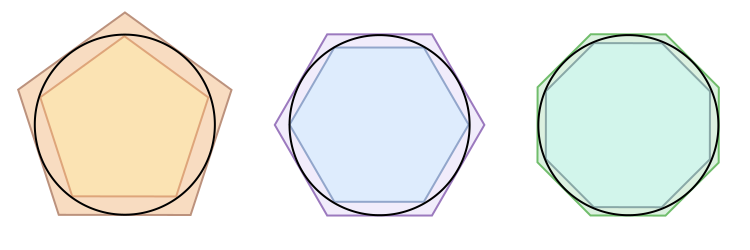
\includegraphics[scale=0.4]{images/archimedes}
		\caption{Aproximaciones de $\pi$ mediante polígonos regulares.}
		\label{fig:Arquimedes}
\end{figure}

Al calcular los perímetros de estos polígonos
Arquímedes logró demostrar que
\[
	3,1408=\frac{223}{71}<\pi<\frac{22}{7}=3,1429
\]

En otras civilizaciones encontramos distintas aproximaciones para el número
$\pi$. En la matemática china, por ejemplo, nos encontramos con que $\pi$ era
aproximado por $3,1547$ y también por $\sqrt{10}$. Cerca del año 265 el
matemático chino Liu Hui divisó un algoritmo que le permitió aproximar $\pi$
como $3,1416$.  En el año 480 el matemático chino Zu Chongzhi mostró que 
\[
	3,1415926<\pi<3,1415927
\]
y sugirió que $\pi$ fuera aproximado por los racionales $355/113$ y $22/7$. 

Creemos que el primer matemático que utilizo la letra griega $\pi$ para denotar
al cociente entre la circunferencia y el diámetro fue William Jones en 1706.
Euler utilizó la letra $\pi$ para denotar esta famosa constante en su libro de
1736 sobre mecánica. 

La aparición de las series infinitas en los siglos XVI y XVII permitieron
obtener mejores aproximaciones para $\pi$ que aquellas encontradas por
Arquímedes mediante métodos geométricos. 

\label{Vieta}
\label{Wallis}
En 1593 Vieta encontró la
expresión
\[
	\frac{2}{\pi}=\dfrac{\sqrt{2}}{2}\dfrac{\sqrt{2+\sqrt{2}}}{2}\dfrac{\sqrt{2+\sqrt{2+\sqrt{2}}}}{2}\cdots
\]
y en 1655 Wallis encontró una expresión que involucra productos infinitos:
\[
	\frac{\pi}{2}=\frac21\frac23\frac43\frac45\frac65\frac67\frac87\frac89\cdots
\]

\label{LeibnizGregory}
El cálculo de Leibniz y Newton permitió obtener muchas otras expresiones
infinitas que involucran al número $\pi$. Gregory y Leibniz, alrededor del año
1670, descubrieron, independientemente la expresión
\[
	\frac{\pi}{4}=1-\frac13+\frac15-\frac17+\cdots
\]
al especializar en un cierto valor la expansión en serie 
\[
	\arctan x=x-\frac{x^3}{3}+\frac{x^5}{5}-\cdots,
\]
encontrada por primera vez en la matemática india en el siglo XV.

En 1761 Lambert demostró que $\pi$ es irracional.  La demostración que dio
Lambert sobre la irracionalidad de $\pi$ es bastante difícil, se basa en la
siguiente expansión para la tangente:
\[
	\tan(x)=\dfrac{x}{1-\dfrac{x^2}{3-\dfrac{x^2}{5-\dfrac{x^2}{7-\cdots}}}}
\]

Hermite dio otra demostración de la irracionalidad de $\pi$ en 1873, y esta
demostración es mucho más sencilla que aquella encontrada por Lambert. 

En 1941 Niven encontró una demostración muy breve y sencilla, que bien podría
darse en cualquier curso de cálculo. Esta demostración utiliza ingeniosamente
algunas de las ideas de Hermite. Veamos la demostración de la irracionalidad de
$\pi$ encontrada por Niven:

\begin{theorem}
	\index{Irracionalidad!de $\pi$}
	El número $\pi$ es irracional.	
\end{theorem}

\begin{proof}
	Supongamos que $\pi=a/b$ con $a$ y $b$ enteros positivos. Sea 
	\[
		f(x)=\frac{x^n(a-bx)^n}{n!}.
	\]

	Primero observemos que $f$ es un polinomio de la forma
	$f(x)=\frac{1}{n!}\sum_{j=n}^{2n}c_jx^j$, donde los $c_j$ son números
	enteros. En efecto, por la fórmula del binomio, 
	\[
		f(x)=\frac{1}{n!}\sum_{j=0}^n\binom{n}{j}a^jx^{2n-j},
	\]
	que puede reescribirse como $f(x)=\sum_{j=n}^{2n}c_jx_j$ para ciertos
	enteros $c_j$.  En particular, $f^{(k)}(0)=\frac{k!}{n!}c_k\in\Z$ si $n\leq
	k\leq 2n$. Como además $f(x)=f(a-bx)$, se demuestra fácilmente por
	inducción que $f^{(k)}(x)=(-b)^kf^{(k)}(a-bx)$ para todo $k$. Luego
	$f^{(k)}(\pi)=(-b)^kf^{(k)}(0)$ para todo $k$. Esto implica que si definimos 
	\[
	F(x)=f(x)-f^{(2)}(x)+f^{(4)}(x)-\cdots+(-1)^nf^{(2n)}(x), 
	\]
	entonces $F(0)+F(\pi)\in\Z$. 

	Como $f(x)$ es un polinomio de grado $2n$, tenemos que $f^{(2n+2)}(x)=0$ y
	luego $F''(x)+F(x)=f(x)$.  Un cálculo directo muestra entonces que
	\[
		\frac{d}{dx}\left( F'(x)\sin x-F(x)\cos x\right)=(F''(x)+F(x))\sin x=f(x)\sin x.
	\]
	En consecuencia, 
	\[
		\int_0^\pi f(x)\sin xdx=F(0)+F(\pi)\in\Z.
	\]
	En el intervalo $(0,\pi)$, las funciones $f(x)$ y $\sin x$ son estrictamente positivas.
	Sabemos además que en este intervalo vale que $0\leq x(a-bx)=xa-bx^2\leq
	\pi a$. 
	Luego
	\[
		0<\int_0^\pi f(x)\sin xdx\leq \int_0^\pi \frac{(\pi a)^n}{n!}dx=\frac{(\pi a)^n}{n!}\pi.
	\]
	Pero $\displaystyle{\lim_{n\to\infty}\frac{\pi^{n+1}a^n}{n!}=0}$, una contradicción.
\end{proof}

%En 1760 Lambert y Riccati, en forma independiente, introdujeron las funciones
%hiperbólicas y estudió algunas de sus propiedades. 

Quizá sea este un buen momento para permitirnos ir hacia otro tópico importante
en la historia de la matemática. Antes de irnos, mencionaremos una fantástica
fórmula encontrada por Euler en 1734: 
\begin{equation}
	\label{eq:pi^2/6}
\sum_{n=1}^{\infty}\frac{1}{n^2}=\frac{\pi^2}{6}.
\end{equation}

No vamos a demostrar en detalle esta fórmula pero sí mencionaremos brevemente
cómo podríamos demostrarla utilizando simplemente técnicas de cálculo. La idea
es calcular una cierta integral de dos formas distintas e igualar estos
resultados. La integral a calcular es 
\[
		I=\int_0^1\int_0^1 \frac{1}{1-xy}dxdy.
	\]
Como dijimos, debemos calcular $I$ de dos formas distintas.  Un método para
calcular esta integral consiste en escribir el integrando como una serie y
realizar algunos cálculos sencillos: 
	\begin{align*}
		I&=\int_0^1\int_0^1 \sum_{n\geq0}(xy)^ndxdy\\
		&=\sum_{n\geq0}\int_0^1\int_0^1 (xy)^ndxdy\\
		&=\sum_{n\geq0}\int_0^1x^ndx\int_0^1y^ndy\\
		&=\sum_{n\geq0}\frac{1}{n+1}\frac{1}{n+1}\\
		&=\sum_{n\geq1}\frac{1}{n^2}.
	\end{align*}
Otra forma de calcular $I$ involucra realizar algún ingenioso cambio de
variables. En efecto, si calculamos $I$ con el cambio de variables
$u=\frac{x+y}{2}$ y $v=\frac{-x+y}{2}$, podremos demostrar la fórmula
encontrada por Euler. 
%	\begin{align*}
%		I&=4\int_0^{1/2}\left(\int_0^u\frac{dv}{1-u^2+v^2}\right)du+4\int_{1/2}^1\left(\int_0^{1-u}\frac{dv}{1-u^2+v^2}\right)du\\
%		&=\dots
%	\end{align*}

\begin{exercise}
	Demuestre la fórmula~\eqref{eq:pi^2/6}.
\end{exercise}

Veamos cómo fue que Euler encontró la fórmula~\eqref{eq:pi^2/6}. Una de las
fórmulas de Newton para polinomios nos permite escribir polinomios como
\[
	1-\alpha_1x+\alpha_2x^2+\cdots+(-1)^k\alpha_kx^k
	=\left(1-\frac{x}{a_1}\right)\left(1-\frac{x}{a_2}\right)\cdots\left(1-\frac{x}{a_k}\right),
\]
donde 
\begin{align*}
	\alpha_1&=\frac{1}{a_1}+\frac{1}{a_2}+\cdots\\
	\alpha_2&=\frac{1}{a_1a_2}+\frac{1}{a_1a_3}+\cdots
\end{align*}
y así sucesivamente. En particular, 
\begin{align*}
	&\frac{1}{a_1^2}+\frac{1}{a_2^2}+\cdots = \alpha_1^2-2\alpha_2,\\
	&\frac{1}{a_1^3}+\frac{1}{a_2^3}+\cdots = \alpha_1^3-3\alpha_1\alpha_2+3\alpha_3,\\
	&\frac{1}{a_1^4}+\frac{1}{a_2^4}+\cdots = \alpha_1^4-4\alpha^2_1\alpha_2+4\alpha_1\alpha_3-4\alpha_4,
\end{align*}
y así sucesivamente. 

La arriesgada idea de Euler es la de utilizar una extensión de esta última
fórmula pero para series de la forma
\[
	1-\alpha_1x+\alpha_2x^2+\cdots,
\]
De hecho, en el caso particular de la serie
\[
	1-\sin x=1-x+\frac{x^3}{3!}-\frac{x^5}{5!}+\frac{x^7}{7!}-\cdots
\]
tenemos que, como la función $x\mapsto 1-\sin x$ tiene ceros en 
\[
	\frac{\pi}{2},\frac{\pi}{2},-\frac{3\pi}{2},-\frac{3\pi}{2},\frac{5\pi}{2},-\frac{7\pi}{2},-\frac{7\pi}{2},\dots
\]
la fórmula para $\alpha_1$ que vimos antes implica que
\[
	\frac{4}{\pi}\left(1-\frac13+\frac15-\cdots\right)=1,
\]
de donde inmediatamente se obtiene la fórmula de Gregory--Leibniz.  

Si utilizamos la
fórmula para $\alpha_1^2-2\alpha_2$ obtenemos además 
\[
	\frac{8}{\pi^2}\left(1-\frac13+\frac15-\cdots\right)=1.
\]
Luego
\begin{align*}
	\sum_{n=1}^\infty\frac{1}{n^2} &= \sum_{n=1}^\infty\frac{1}{(2n)^2}+\sum_{n=0}^\infty\frac{1}{(2n+1)^2}=\frac14\sum_{n=1}^\infty\frac{1}{n^2}+\frac{\pi^2}{8},
\end{align*}
de donde se deduce inmediatamente la fórmula~\eqref{eq:pi^2/6}.
Esta fórmula nos permite entender por qué algunas civilizaciones aproximaban a
$\pi$ con el número $\sqrt{10}$. Primero, observemos que 
\[
	\sum_{n=1}^\infty\frac{1}{n^2}=1+\sum_{n=2}^\infty\frac{1}{n^2}<\sum_{n=2}^\infty\frac{4}{4n^2-1}.
\]
Para sumar esta última serie, observamos que
\[
	\frac{4}{4n^2-1}=\frac{4}{(2n-1)(2n+1)}=\frac{2}{2n-1}-\frac{2}{2n+1}=\frac{2}{2n-1}-\frac{2}{2(n+1)-1}.
\]
Luego 
\[
	\sum_{n=1}^\infty\frac{1}{n^2}<1+\left(\frac23-\frac25\right)+\left(\frac25-\frac27\right)+\left(\frac27-\frac29\right)+\cdots=1+\frac23=\frac53
\]
y entonces $\pi^2<6(5/3)=10$. El error es bastante pequeño pues 
\begin{align*}
	\frac53-\sum_{n=1}^\infty\frac{1}{n^2}
	&=\sum_{n=2}^\infty\left(\frac{4}{4n^2-1}-\frac{1}{n^2}\right)\\
	&=\sum_{n=2}^\infty\frac{1}{n^2(4n^2-1)}
	\leq\sum_{n=2}^\infty\frac{16}{60x^4}
	<\int_1^{\infty}\frac{16}{60}t^4dt=\frac{16}{180}.
\end{align*}

Tal como hizo Euler, pueden usarse fórmulas similares para encontrar otras series 
que involucren potencias de $\pi$ como por ejemplo
\[
	1+\frac{1}{2^4}+\frac{1}{3^4}+\cdots=\frac{\pi^4}{90}.
\]


\subsection*{El teorema del binomio}
\index{Teorema!del binomio}

El teorema del binomio fue mencionado en la demostración de Niven de la
irracionalidad de $\pi$. El resultado afirma que para un entero positivo $n$ vale la siguiente fórmula
\[
	(x+y)^n=\sum_{k=0}^n\binom{n}{k}x^ky^{n-k},
\]
donde
\[
	\binom{n}{k}=\frac{n!}{k!(n-k)!}
\]
son los coeficientes binomiales. Una versión más general afirma si $|x|<|y|$ y además 
$r\in\C$, entonces vale la siguiente fórmula 
\[
	(x+y)^r=\sum_{k=0}^\infty\binom{r}{k}x^{k}y^{r-k},
\]
donde 
\[
	\binom{r}{k}=\frac{r(r-1)\cdots (r-k+1)}{k!},
\]
expresión que coincide con los coeficientes binomiales si $n$ es un entero
positivo. 

\begin{example}
	Una aplicación sencilla de la fórmula del binomio nos da la siguiente fórmula, válida 
	para todo $x$ tal que $|x|<1$:
	\begin{align*}
		(1+x)^{-1}&=1-x+x^2-x^3+x^4+\cdots
	\end{align*}
\end{example}

%\begin{exercise}
%	Demuestre que para $x$ tal que $|x|<1$ valen las siguientes fórmulas:
%	\begin{align*}
%		\sqrt{1+x}&=1+\frac12x-\frac18x^2+\frac{1}{16}x^3-\frac{5}{128}x^4+\cdots,\\
%		\frac{1}{\sqrt{1+x}}&=1-\frac12x+\frac38x^2-\frac{5}{16}x^3+\frac{35}{128}x^4-\cdots
%	\end{align*}
%\end{exercise}

La primera aparición escrita de algo similar al
teorema del binomio aparece en uno de los libros de Euclides, donde se
demuestra que vale la fórmula
\[
	(a+b)^2=a^2+b^2+2ab.
\]
Euclides también demuestra una identidad similar:
\[
	a^2+b^2=2ab+(a-b)^2.
\]

Según Coolidge~\cite{MR28222}, Euclides estaba en condiciones de obtener
fácilmente la fórmula para el cubo de un binomio pero en épocas de Euclides se
priorizaba la claridad y la precisión y no se intentaba obtener resultados en
la forma más general posible como pasa en la matemática de la actualidad.  

Se cree que en el siglo V el matemático indio Aryabhata conocía la fórmula para el
cubo de un binomio, y que esta fórmula tenía interés dado que era utilizada
para aproximar raíces cúbicas. No sabemos si la matemática india estaba
interesada en otras potencias de un binomio, pero posiblemente este problema no
resultara de interés ya que carecía de aplicaciones prácticas. 

Alrededor del
año 1300 varios matemáticos chinos mostraron interés en lo que hoy
--injustamente-- conocemos como el triángulo de Pascal, que no es otra cosa que
la representación de los coeficientes binomiales ordenados en forma de
triángulo: 

\begin{center}
\begin{tabular}{rccccccccc}
    &    &    &    &  1\\\noalign{\smallskip\smallskip}
    &    &    &  1 &    &  1\\\noalign{\smallskip\smallskip}
    &    &  1 &    &  2 &    &  1\\\noalign{\smallskip\smallskip}
    &  1 &    &  3 &    &  3 &    &  1\\\noalign{\smallskip\smallskip}
  1 &    &  4 &    &  6 &    &  4 &    &  1\\\noalign{\smallskip\smallskip}
\end{tabular}
\end{center}

Se sabe que esta configuración de números era ya bien conocida desde tiempo antes, en
particular en la matemática china y árabe. Varios historiadores creen que los
matemáticos chinos sabían además cómo calcular elevadas potencias de un binomio. 

En 1544 un monje alemán llamado Stifel publicó \emph{Arithmetica integra}, un
importante tratado sobre aritmética donde aparece una lista de números enteros
que hoy interpretamos como la fórmula
\[
	\binom{n}{k}=\binom{n-1}{k}+\binom{n-1}{k-1}.
\]

El tratado de Stifel contiene además importantes avances en 
notación matemática (escribir la multiplicación por juxtaposición, por ejemplo,
o el uso del término ``exponente'' para las potencias, así como también
la introducción del término ``coeficiente binomial''), contiene una tabla de
potencias de dos que no es sino una forma precaria de una tabla de logaritmos,
trata a los números negativos de la misma forma que trata a los números
positivos, sin ninguno de los prejuicios que los negativos enfrentaban en
aquellos tiempos. Stifel además estudió en su tratado propiedades de los
números irracionales y concluye que tales números son necesarios en la
matemática. 

En 1655 Pascal publicó un tratado donde figuran muchos resultados sobre los
coeficientes binomiales y  utilizó además estos resultados para resolver
problemas de la teoría de probabilidades. Fue en esta publicación donde Pascal
observó que la cantidad de subconjuntos de $k$ elementos de un conjunto de $n$
elementos es igual a 
\[
	\binom{n}{k}=\frac{n!}{k!(n-k)!},
\]
aunque aparentemente esta fórmula era ya conocida por Briggs en 1620.  

En 1708
Pierre Rémond publicó un tratado sobre los juegos de azar y fue precisamente en
aquel libro donde le atribuyó a Pascal la invención del triángulo formado por
los coeficientes binomiales. 

Años más tarde, Gregory e independientemente Newton consideraron necesario
poder calcular potencias fraccionarias de binomios y obtuvieron algunos
resultados. Newton, por ejemplo, encontró la fórmula
\begin{align*}
	(1-x^2)^{1/2}&=1-\frac{x^2}{2}-\frac{x^4}{8}-\frac{x^6}{16}\cdots,
\end{align*}
aunque no sabemos exactamente cuál fue el método que le permitió obtener esa y
otras fórmulas similares. 

Coolidge afirma que no es justo decir que Newton
demostró el teorema del binomio, ya que, según parece, el gran genio inglés
simplemente mostró que en ciertos casos la fórmula sugerida por el teorema
del binomio daba el resultado correcto si el exponente era un cierto número
racional. 

Para encontrarnos con algunos de los primeros pasos hacia obtener una
demostración rigurosa del teorema del binomio debemos saltar hacia 1742, año en
un matemático italiano de apellido Salvemini publicó un trabajo donde menciona
que todos conocen al teorema de Newton pero nadie parece haberlo demostrado.
Demuestra entonces el teorema del binomio después de haber distinguido tres
posibles casos: a) el exponente es un entero positivo, b) el exponente es una
fracción positiva, y por último c) el exponente es negativo. Ese mismo año una
demostración mucho más breve e ingeniosa aparece en \emph{A treatise on
Fluxions}, un libro de 736 páginas escrito por el matemático escocés Colin
Maclaurin. La demostración de Maclaurin es más o menos así: Supongamos que
queremos calcular $(1+x)^n$, donde $n$ es un número racional positivo o
negativo. Escribimos entonces
\[
	(1+x)^n=1+Ax+Bx^2+Cx^3+\cdots
\]
Al derivar ambos miembros de la igualdad obtenemos la identidad
\begin{equation}
	\label{eq:Maclaurin}
	n(1+x)^{n-1}=A+2Bx+3Cx^2+\cdots
\end{equation}

Al reemplazar $x$ por cero en esta igualdad, obtenemos que $A=n$. Si derivamos
la igualdad~\eqref{eq:Maclaurin} para luego evaluar la nueva identidad en
$x=0$, podremos calcular explícitamente el valor de $B$. El resto de los
coeficientes se obtendrá entonces muy fácilmente mediante esta técnica que
involucra el cálculo de derivadas. Seguramente muchos lectores estarán algo incómodos, ya que 
en esta ``demostración'' hay varias cosas
que falta justificar, de eso no hay duda. Un agujero particularmente importante
es el de la convergencia. ¡Debemos asegurarnos de que las series convergen!
Este problema era reconocido por Maclaurin, pero no fue capaz de resolverlo. El
primer matemático capaz de resolver los problemas de convergencia 
en relación al teorema del binomio fue Abel y lo hizo en
1826. 


% numeros de bernoulli

